\documentclass[12pt]{article}
\usepackage[a4paper,margin=2.5cm]{geometry}
\usepackage{amsmath,amssymb}
\usepackage{graphicx}
\usepackage{subcaption}
\usepackage{booktabs}
\usepackage{array}
\usepackage{setspace}
\usepackage[round]{natbib}
\setcitestyle{aysep={,},yysep={,}}
\usepackage{url}
\usepackage[hidelinks]{hyperref}
\usepackage[running]{lineno}
\hypersetup{pdftitle={From photograph to loom draft: self-checking digital records of Koh Yo hand-woven textile patterns},pdfauthor={Thanathorn Kittikant and Nitipong Praphaphankul}}
\graphicspath{{figures/panels/}}
\setcounter{secnumdepth}{0}
\renewcommand{\figurename}{Figure}
\newcolumntype{L}[1]{>{\raggedright\arraybackslash}p{#1}}
\begin{document}
\onehalfspacing
\begin{center}
{\LARGE\bfseries From photograph to loom draft: self-checking digital records of Koh Yo hand-woven textile patterns\par}
\vspace{1em}
{\large Thanathorn Kittikant$^{a}$ and Nitipong Praphaphankul$^{b,*}$\par}
\vspace{0.6em}
{\small $^{a}$Department of Industrial Design, Faculty of Architecture, Chulalongkorn University, Bangkok, Thailand\\
$^{b}$Center of Excellence in Urban Strategies and Healthy Cities, Faculty of Architecture, Chulalongkorn University, Bangkok, Thailand\\
$^{*}$Corresponding author: nitipong.pr@chula.ac.th\par}
\end{center}
\vspace{0.5em}
\linenumbers
\section{Abstract}
The supplementary-weft patterns of Koh Yo cloth, Songkhla, Thailand, exist only in the loom set-ups and memories of a small number of weavers; no written drafts exist. This paper presents a method that turns an ordinary hand-held photograph of such a cloth into a clean pattern tile and a cell-level weaving draft in loom formats, together with checks that state how far the record can be trusted. The cloth's own repeating structure is used to correct tilt, perspective and folds, to average all repeats into one tile, and to read the draft from it. On five Koh Yo patterns photographed in the field the pattern repeat was found on all five cloths, where the standard rule found it on one; the disagreement between repeats fell by 24\% to 53\%; and on artificial cloth of known structure the draft came back with 99.8\% to 100\% agreement. Four of the five drafts can be projected onto the weaver's stated heddle count by changing only 2.4\% to 3.8\% of cells, against 10\% to 25\% for a random draft, and a reading rule drawn from the checks places three records ready for use, one for confirmation by the weaver and one for a closer photograph. The method needs no equipment beyond a camera, runs in seconds, and gives conservators and weaving communities a verifiable record of a pattern and guidance for photographing cloth in the field.

\noindent\textbf{Keywords:} conservation documentation; textile structure; intangible cultural heritage; hand-woven textiles; supplementary weft; Thailand; weaving draft; image analysis

\section{Introduction}

Koh Yo, an island community in Songkhla Lake in southern Thailand, has woven cotton and silk cloth since the Ayutthaya period, and its supplementary-weft patterns, such as Ratchawat, Luk Kaeo and Dok Phakakrong, are listed by the Prince of Songkla University southern information database as a living repertoire of more than fifty named designs \citep{psu_kohyo}. The patterns are not written down. They live in the heddle set-up of a hand loom, in the way a weaver lifts the shafts, and in the memory of the weaving groups of two villages on the island \citep{psu_kohyo,conway1992,prangwatthanakun1987}. The UNESCO convention on intangible heritage names documentation, alongside transmission, among the measures that safeguard a living practice \citep{unesco2003}, and a record of a woven pattern is only useful when its accuracy is known \citep{pavlidis2007}.

The problem is familiar to textile conservators. Collections hold woven pieces whose structure must be recorded before handling, display or loan; support or replacement fabrics must sometimes be woven to match a pattern; and source communities increasingly ask museums to help keep a weaving tradition alive. In each case the useful record is not only an image but a description of how the cloth was made, which is normally obtained by counting threads under magnification, following the conventions of \citet{emery1980} and \citet{burnham1980}, or by asking the weaver. Both are slow, and the second is impossible once the weaver has gone. A method that turns a photograph into a weaving draft, and states how reliable that draft is, would let a conservator or a community member document a pattern in minutes, without special equipment and without handling the object beyond laying it flat.

Image analysis of woven and printed textiles has a long history in textile engineering and computer vision, but its inputs and outputs differ from what documentation needs. Thread-level weave recognisers \citep{kang1999,kuo2004,xin2009,pan2011,hussain2020,meng2021}, reviewed by \citet{zhang2013} and \citet{zhang2016}, work on flat-bed scans or macro images that resolve each thread with about 12 or more pixels \citep{meng2021}, which a hand photograph of a whole cloth does not reach. Repeat extraction for printed fabric \citep{tavanai2006,kuo2008,xiang2020,xiang2022,ayyurek2026} and lattice detection for near-regular textures \citep{liu2004pami,liu2004siggraph,hays2006,park2009,liu2015,albert2015} find the repeat but stop at the image; none produces a loom draft or checks its output against the maker of the object. Micro-CT reconstructs yarn geometry in great detail \citep{ying2025,tang2024,cao2025} at a cost no field survey can pay. An earlier proof of concept by the authors converted a flat pattern graphic into a TC2 Jacquard file; it assumed that one pixel is one thread and that the source is flat, neither of which holds for a photograph of cloth taken by hand.

This paper asks two questions for five Koh Yo patterns. First, how can the geometry of a hand photograph, its tilt, perspective, folds and uneven light, be removed so that the pattern repeat is sharp? Second, how can the correctness of the extracted draft be judged when no ground-truth draft exists? The answer to the first is a lattice-first geometry recovery that uses the cloth's own repetition in place of a calibration target, with a new rule for finding the repeat that succeeds where the standard rule fails on these cloths. The answer to the second is a set of checks that every record carries: against the photograph, against itself, against artificial cloth of known structure, and against the weaver's own heddle count. For practice, the paper gives a reading rule that places each record as ready for use, for confirmation by the weaver or for a closer photograph, guidance for photographing a cloth in the field, both in the Discussion, and the code, photographs and loom files openly.

\section{Terms used}

The image-processing terms the paper needs are explained in Table~\ref{tab:terms}; weaving terms follow \citet{emery1980} and \citet{burnham1980}. Each stage of the method is also summarised in plain words at the start of its subsection, with the parameter values collected at the end of the Method.

\begin{table}[htbp]
\caption{Terms used in this paper.}
\label{tab:terms}
\small
\renewcommand{\arraystretch}{1.1}
\begin{tabular}{L{3.2cm}L{11.3cm}}
Term & Meaning in this paper \\ \midrule
Repeat & The smallest rectangle of the pattern that, laid side by side, reproduces the whole cloth. \\
Pattern cell & The smallest unit of the design: one float of supplementary weft over one group of warp ends. The draft is a grid of cells, each either float or ground. The number of threads in a cell is not measured by the method. \\
Shaft, heddle & A shaft is a frame of heddles that lifts a chosen set of warp ends together. The weavers of Koh Yo describe their patterns by the number of pattern heddles; the draft is described by the number of pattern shafts it needs, and the two are compared. \\
Weaving draft & The instructions for a loom: the threading assigns each warp end to a shaft, the tie-up links treadles to shafts, the treadling lists the treadle for each pick of weft, and the drawdown is the pattern that results. \\
WIF, TC2 & WIF is the plain-text draft format read by most weaving software; the TC2 is a digital Jacquard hand loom that weaves from an image file. \\
Autocorrelation & A map of how well the image matches a copy of itself shifted by every possible amount; its peaks reveal the repeat. \\
Mean tile & The average of all the aligned repeats: one clean colour image of a single repeat. \\
Measured draft & The two-colour draft obtained by thresholding the mean tile on its lightness and reading it on the cell grid; Otsu's method chooses the threshold automatically. \\
Regularised draft & An interpretation of the measured draft in which only those mirror, rotation and shift symmetries that the draft already shows are enforced; a simpler draft for the weaver to accept or reject. \\
SSIM, CIEDE2000 & Standard measures of how closely a reconstruction matches the photograph: SSIM scores similarity of structure between 0 and 1, and CIEDE2000 is a colour difference in units where one unit is about the smallest difference a viewer can see. \\
Round trip & Rendering an artificial photograph of cloth from a known draft, analysing it, and checking whether the known draft comes back. \\
\end{tabular}
\end{table}

\section{Koh Yo cloth and the five patterns}

Koh Yo cloth is woven on a treadle loom introduced to the island in 1939 after Chinese teachers replaced the older bamboo hand loom \citep{psu_kohyo}. The ground is a plain or alternating-colour weave on two shafts, and the pattern is raised by supplementary floats controlled by additional shafts; the database records patterns on two to twelve shafts and notes that more shafts give finer, more expensive designs \citep{psu_kohyo}. The visible pattern is therefore a two-colour structure, float visible or not, at the scale of a pattern cell, laid over a coloured ground. \citet{grunbaum1980} give the geometric background for such periodic fabrics. The cloth was traditionally cotton, grown on the island until the Second World War, and is now also woven in silk, artificial silk and rayon with natural or synthetic dyes; the favoured colourings are white with red, sometimes with black or yellow \citep{psu_kohyo}. A weaver produces four to seven yards a day depending on how hard the reed is beaten, which also sets the density of the cloth \citep{psu_kohyo}.

The five patterns are listed in Table~\ref{tab:patterns} and shown in Fig.~\ref{fig:photos}. Each is a new cloth, photographed by the authors on the island with a hand-held camera; no historic or worn piece was included, so the method is tested on cloth in good condition only. For each cloth the weaver gave the pattern name and the number of pattern heddles used to weave it, four for three patterns and eight for two. The count refers to the pattern heddles, and the shafts counted for the drafts in this paper are likewise pattern shafts, since the cell draft records the supplementary floats and not the two shafts of the ground weave. The photographs are between 882 and 1196 pixels wide and were taken by hand, so they contain rotation, perspective, uneven light and in one case a slight fold. They are deliberately typical of what a field survey produces.

The patterns are the heritage of the weaving community of Koh Yo. The photographs and the derived pattern files are released under a Creative Commons Attribution licence that asks for the weavers of Koh Yo to be credited, and the drafts are offered as a documentation aid for the community and for conservators, not as a substitute for the weavers' knowledge.

\begin{table}[htbp]
\centering\footnotesize\setlength{\tabcolsep}{3pt}
\caption{The five patterns: weaver's pattern-heddle count, photograph and rectified sizes in pixels, and repeats in the rectified image (size divided by period).}
\label{tab:patterns}
\begin{tabular}{llccccc}
Id & Pattern & Heddles & Photograph & Rectified & Repeats & Repeats \\
 & & & (pixels) & (pixels) & across & down \\
\midrule
P1 & Ratchawat & 4 & 960 $\times$ 720 & 846 $\times$ 606 & 10.6 & 7.1 \\
P2 & Dok Phakakrong & 8 & 1175 $\times$ 541 & 1041 $\times$ 407 & 20.4 & 4.1 \\
P3 & Dok Rotsukhon with Luk Kaeo & 8 & 882 $\times$ 580 & 782 $\times$ 480 & 5.5 & 3.3 \\
P4 & Kamphaeng & 4 & 884 $\times$ 550 & 750 $\times$ 416 & 7.0 & 4.0 \\
P5 & Luk Kaeo & 4 & 1196 $\times$ 848 & 980 $\times$ 632 & 8.8 & 3.1 \\
\end{tabular}
\end{table}

\begin{figure}[htbp]
\centering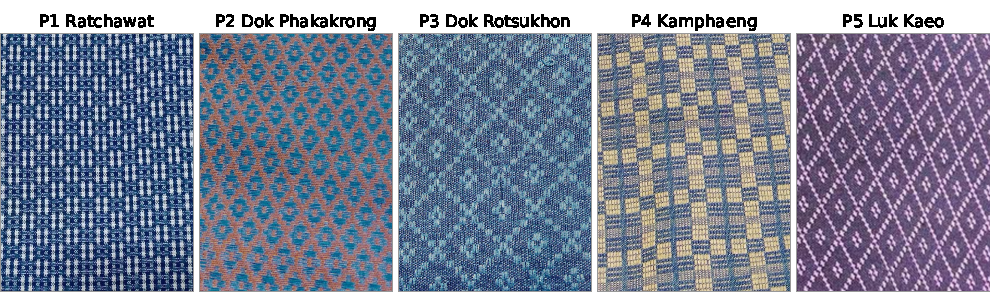
\includegraphics[width=\textwidth]{sic_photos}
\caption{The five cloths as photographed by hand in the field, centre-cropped to one aspect: P1 Ratchawat, P2 Dok Phakakrong, P3 Dok Rotsukhon with Luk Kaeo, P4 Kamphaeng, P5 Luk Kaeo.}
\label{fig:photos}
\end{figure}

\section{Method}

\subsection{Overview}

Fig.~\ref{fig:flow} shows the method in three steps. The first straightens the photograph using the cloth's own repeat, so that the pattern lattice is square and uniform. The second averages all the repeats into a single clean tile and reads a two-colour draft from it on a grid of pattern cells. The third turns the cell draft into loom instructions, writes the WIF and TC2 files, and collects the checks. The whole run takes about twenty seconds for the five patterns on a laptop; every number in this paper is read from the results files written by the code.

\begin{figure}[htbp]
\centering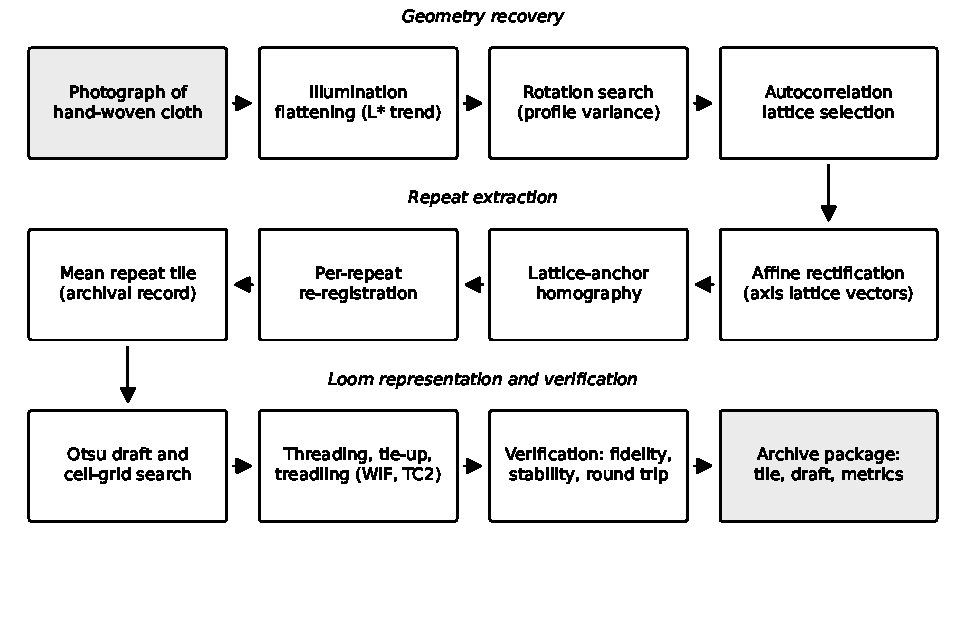
\includegraphics[width=\textwidth]{fig01_flowchart}
\caption{The method: the photograph is straightened with its own repeat, the repeats are averaged into a tile and read as a cell draft, and the draft is factored for the loom and checked against the photograph, artificial cloth and the weaver's heddle count.}
\label{fig:flow}
\end{figure}

\subsection{Straightening the photograph}

In plain words, this step evens out the lighting, turns the cloth straight, finds how far the pattern repeats, and removes the perspective of the camera and the small distortions of a cloth that is not perfectly flat. The photograph is converted to the CIELAB colour space, which separates lightness from colour. The lightness is divided by a heavily blurred copy of itself and rescaled to its original mean, a flattening in the spirit of retinex \citep{land1971} that removes the darkening towards the corners and the shadow of a fold without changing the colours. Rotation is found by trying every angle between minus eight and eight degrees and keeping the one at which the pixel sums along rows and columns vary most strongly, which happens only when weft and warp run exactly along the image axes.

The repeat is then read from the autocorrelation of the central part of the image, after light blurring to suppress yarn texture. The standard rule of the texture literature takes the two shortest strong peaks as the repeat \citep{liu2004pami,liu2004siggraph}. On supplementary-weft cloth this fails, because the small elements inside a motif, the dashes of Ratchawat for example, correlate more strongly with each other than the whole repeat does with its neighbour. The rule introduced here, the shell rule, asks a simple question of each candidate repeat: if the pattern really repeats by this step, it must also match itself at every neighbouring multiple of the step, two steps away as well as one. A candidate is scored by its weakest match among the eight nearest multiples, and checked at the next ring. A true repeat is strong at all of them; a correlation between parts of a motif fails two steps away, as Fig.~\ref{fig:mshell} shows for Ratchawat.

\begin{figure}[htbp]
\centering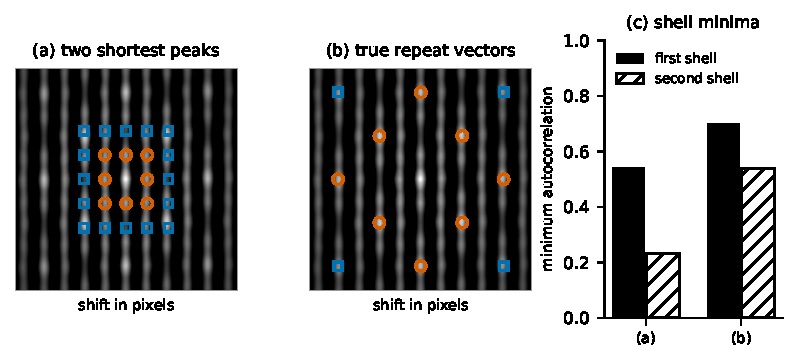
\includegraphics[width=\textwidth]{method_shell}
\caption{The shell rule on P1. Autocorrelation with the first shell (circles) and second shell (squares) of the two shortest peaks (a) and of the true repeat vectors (b); the minimum over each shell (c). The shortest peaks collapse at the second shell; the true repeat does not.}
\label{fig:mshell}
\end{figure} Among well-scoring grids the one with the smallest cell is kept, so that a double-size repeat is not chosen. The lattice is called centred when the pattern also repeats at half the diagonal, the diamond arrangement typical of supplementary-weft work.

Shear from oblique viewing is removed by a linear stretch and skew that brings the two measured repeat directions exactly onto the image axes. Perspective is removed next: a small template of the central three by three repeats is searched for across the image, its best match is recorded at 35 anchor positions working outwards from the centre, and the perspective transformation, or homography \citep{hartley2003}, that maps the anchors onto their positions on a flat cloth is fitted by a procedure that ignores mismatched anchors \citep{fischler1981}. It is applied only when enough anchors are found and when the repeat measured afterwards agrees with the repeat measured before; otherwise the image is kept as it was. The repeat period is then confirmed by a second, independent estimate: the image is folded at every candidate period near the autocorrelation value, and the period at which the individual repeats disagree least with their average is taken. Finally, because cloth is never a plane, every repeat is shifted by up to six pixels to the position where it best matches the running average, and the average is recomputed. The disagreement between the repeats and their average, called the residual, is kept as a map and reported after each stage, because its fall measures what each stage achieves.

\subsection{The pattern tile and the cell draft}

In plain words, this step produces one clean image of a single repeat and turns it into a two-colour grid of cells. The mean tile, the average of all the aligned repeats, is the archival record in colour. It is reduced to two colours by an automatic lightness threshold, Otsu's method \citep{otsu1979}, which separates the pattern floats from the ground, and the two median colours of the classes give the palette. The pixel-level draft is then searched for the coarsest grid of cells that reproduces it: for every candidate number of ends and picks, and for four positions of the grid origin along each axis, the tile is averaged onto the grid, thresholded, enlarged back to pixel size and compared with the pixel draft, and the coarsest grid that reproduces it within 1\% of the best is kept. The search for the origin matters: a cell window that straddles two true cells mixes a float with its ground. Without it, the round trips reported below recovered the exact cell grid in only 2 of 15 cases, against 13 of 15 with it. The search gives the pitch of the pattern cell in pixels, without assuming that one pixel is one thread, and the number of threads in a cell is not measured. Fig.~\ref{fig:mtile} shows the steps on Kamphaeng.

\begin{figure}[htbp]
\centering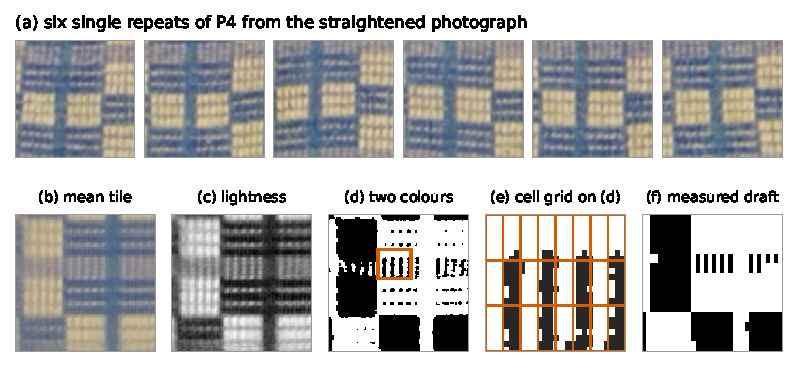
\includegraphics[width=\textwidth]{method_tile2draft}
\caption{From repeats to draft on P4: six single repeats (a), their mean tile (b), its lightness (c), the two-colour draft per pixel (d), the cell grid found by the search drawn over the boxed area of (d) (e), and the measured draft, 34 by 14 cells (f).}
\label{fig:mtile}
\end{figure}

\subsection{The loom draft and the symmetry interpretation}

In plain words, this step writes the loom instructions and offers, beside the measured draft, a cleaned version in which small irregularities that break the pattern's symmetry are removed. The cell draft is factored exactly into a weaving draft: the distinct columns of the grid are the threading classes, so their number is the number of shafts the draft needs; the distinct rows are the treadling classes; and the tie-up is read off at their intersections. The drawdown of the factored draft is checked to equal the cell draft. To see whether the extra shafts are real, the draft is forced onto a given number of shafts, including the weaver's own count, by giving each warp end the nearest of that many column patterns, and the percentage of cells this changes is recorded; this is called the projection cost. For comparison, the same projection is applied to random drafts of the same size and float density. Fig.~\ref{fig:mproj} shows the projection on Kamphaeng.

\begin{figure}[htbp]
\centering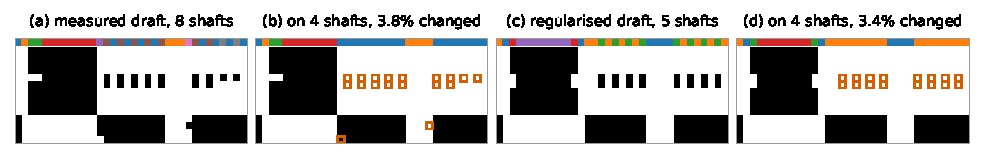
\includegraphics[width=\textwidth]{method_projection}
\caption{Shaft projection on P4. The strip above each draft colours its distinct column patterns, one per shaft; forcing the measured (a) and regularised (c) drafts onto the weaver's four shafts changes the outlined cells (b, d).}
\label{fig:mproj}
\end{figure} The longest floats along picks and ends are counted. The outputs are a WIF file \citep{wif1997} for shaft looms and weaving software, an image of eight by eight repeats with one pixel per cell for the TC2 loom \citep{tc2}, which as a Jacquard loom lifts every end individually and needs no threading, a point-paper chart and the mean tile.

A supplementary-weft pattern is woven with one threading and a short treadling, so it normally has a vertical mirror, a horizontal mirror and a two-fold rotation, and on a centred lattice a half-repeat shift. A photograph does not deliver the draft with these symmetries exactly, because yarn noise, residual misalignment and the weaver's own hand break them cell by cell, and every broken cell adds a threading class and therefore a shaft. A symmetry-regularised draft is therefore produced as an interpretation: each candidate operation is accepted when the draft agrees with its own transform at the best alignment on at least 80\% of cells, the cell lightness is averaged over the accepted operations and thresholded again, and the result is factored as before. The measured draft remains the primary record; the regularised draft, the list of cells it changed, and the measured agreement for each operation are stored beside it. Fig.~\ref{fig:msym} shows the steps on Kamphaeng. Whether the departures from symmetry are noise or real is tested by comparing them with the repeat-to-repeat variation of the averaged tile, as reported below.

\begin{figure}[htbp]
\centering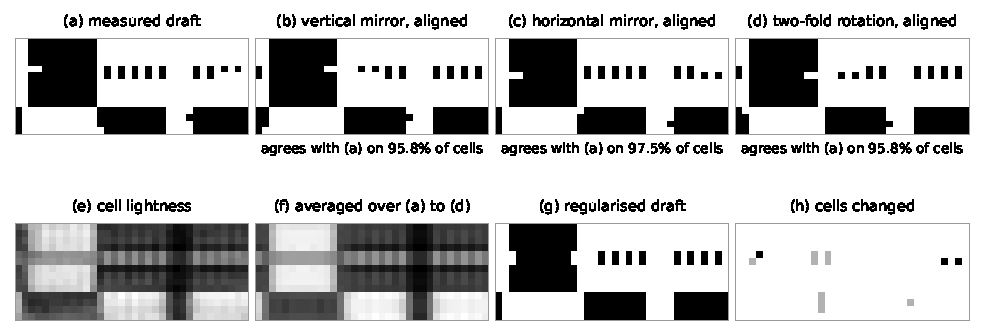
\includegraphics[width=\textwidth]{method_symmetry}
\caption{Symmetry interpretation on P4: measured draft (a), its aligned mirrors and rotation (b to d), cell lightness (e) and its average over (a) to (d) (f), the regularised draft (g) and the cells changed (h).}
\label{fig:msym}
\end{figure}

\subsection{Checks}

In plain words, every record is checked in four ways: against the photograph it came from, against itself, against artificial cloth of known structure, and against the weaver. Fidelity to the photograph is measured by tiling the mean tile and the two-colour draft back over the rectified photograph and comparing them with the structural similarity index SSIM \citep{wang2004}, pixel by pixel and after blurring by two pixels, which is the scale of the motif, together with the colour difference in CIEDE2000 units \citep{sharma2005}. Stability is measured by running the whole method on twelve random crops covering 80\% of each side of the photograph and comparing the repeat found on each crop with the full-image value; this is a crop-stability analysis rather than a bootstrap in the statistical sense, and it reports the spread of the result, not a confidence interval. Round trips render artificial cloth from each extracted cell draft, with yarn shading, vignetting, tilt of 1 to 4 degrees and noise, three cases per pattern, and run the whole method on it; they test whether the extraction can recover a draft of this kind from a photograph with these degradations, not whether the draft of the real cloth is right. Two further synthetic sweeps vary the cell pitch from 2 to 8 pixels and the noise level. Weavability compares the shafts the draft needs, and the cost of projecting it onto the weaver's count, with the weaver's heddle count, which is the only information independent of the photograph. The shell rule is compared with the shortest-vector rule on the full images and on the twelve crops of each.

Nine further techniques from the fabric-analysis, symmetry and machine-learning literature were built into the same framework and tested against the stage each would replace or extend; they are listed with their outcomes at the end of the Results.


\subsection{Parameter values}

Tables~\ref{tab:params} and \ref{tab:params2} list every parameter of the method; all are fixed and none was tuned per pattern.

\begin{table}[htbp]
\caption{Parameter values of the method: geometry, tile and draft.}
\label{tab:params}
\footnotesize
\begin{tabular}{L{4.0cm}L{5.4cm}L{5.2cm}}
Stage & Parameter & Value \\ \midrule
Illumination flattening & Gaussian blur of the lightness trend & standard deviation 45 pixels \\
Rotation search & Angle range and steps & $-8$ to $8$ degrees, coarse 0.5, fine 0.1 \\
Autocorrelation & Window, pre-smoothing, high-pass & Hann window on the central 440 pixels (520 after affine), Gaussian 1.2 pixels, high-pass 25 pixels \\
Peak candidates & Threshold, minimum separation & 0.2 of the central peak, 4 pixels \\
Shell rule & Shells scored, acceptance band, choice among accepted & first shell (coefficients in $\{-1,0,1\}$) minimum and second-shell check; lattices within 80\% of the best score; smallest cell area \\
Centred lattice & Test & autocorrelation at half the diagonal at least half of the axis peaks \\
Perspective correction & Anchors, fit, tolerance, guards & 35 anchors by normalised cross-correlation of the central $3\times3$ repeats; RANSAC homography, 3 pixels; at least 8 anchors, determinant near 1, period change below 5\% \\
Fold refinement & Search band & integer periods within 6\% of the autocorrelation value, parabolic sub-pixel fit \\
Re-registration & Search radius, passes & $\pm 6$ pixels, 2 passes \\
Cell grid & Range, origin phases, knee & 4 ends or picks to one third of the pixel repeat; 4 phases per axis; coarsest grid within 1\% of minimum disagreement \\
Shaft projection & Range, clustering & 2 to 16 shafts; medoid clustering under Hamming distance, 30 iterations \\
Symmetry interpretation & Operations, acceptance, passes & vertical mirror, horizontal mirror, two-fold rotation, half-repeat shift (centred lattice with even cell counts only); agreement at least 80\%; 2 passes \\
\end{tabular}
\end{table}

\begin{table}[htbp]
\caption{Parameter values of the method: checks and tested techniques.}
\label{tab:params2}
\footnotesize
\begin{tabular}{L{4.0cm}L{5.4cm}L{5.2cm}}
Stage & Parameter & Value \\ \midrule
Fidelity & SSIM scales, edge tolerance & pixel scale and Gaussian 2 pixels; Canny edges, 1 pixel \\
Crop stability & Crops, size & 12 random crops, 80\% of each side \\
Round trips & Pitch, tilt, noise & (5, 2.5, 0.04), (7, $-4.0$, 0.08), (4, 1.0, 0.12) pixels per cell, degrees, noise standard deviation; pitch capped so that the repeat stays below 150 pixels \\
Resolution sweep & Pitches & 2, 3, 4, 5, 6, 8 pixels per cell; cases with repeat above 160 pixels skipped (13 of 30) \\
Noise sweep & Levels & 0.02 to 0.25 at 4 pixels per cell (3 for P5) \\
Super-resolution & Registration, grid, floor & phase correlation with 20-fold upsampling; grid 3 times finer; cell pitch at least 2.5 pixels \\
Learned selector & Model, training & gradient-boosted trees on the shell features; 30 synthetic crops; fall back to the rule below probability 0.5 \\
Noise2Noise denoiser & Model & multilayer perceptron, hidden layers 96 and 48, $7\times7$ patch of one repeat predicting the pixel of another \\
Smoothness-prior draft & Model & two-component Gaussian mixture with Ising prior, coupling 0.9, iterated conditional modes \\
Software & Versions and seeds & Python 3.11, NumPy, SciPy, OpenCV, scikit-image and scikit-learn at the versions pinned in the repository; all random seeds fixed in the code \\
\end{tabular}
\end{table}
\section{Results}

\subsection{Geometry and the repeat}

Table~\ref{tab:geom} summarises the geometry of the five photographs and Fig.~\ref{fig:rect} shows them after straightening. Rotation ranged from minus 4.1 to 5.5 degrees and shear from minus 2.1 to 3.0 degrees. The displacement of the anchors from where a flat cloth would put them, before the perspective correction, reached 13.5 pixels on P1, 22.2 on P2 and 51.2 on P5, the most obliquely photographed cloth, while P3 was nearly flat at 8.0 pixels. The repeat period changed by up to 5 pixels between the first and the final estimate, for example from 103.0 to 98.2 pixels vertically on P2, which shows that a repeat measured on an uncorrected hand photograph carries a measurable perspective error.

\begin{table}[htbp]
\centering
\setlength{\tabcolsep}{2.5pt}\scriptsize
\caption{Geometry recovered for each photograph: rotation and shear in degrees, largest anchor drift before perspective correction in pixels, repeat (horizontal by vertical, pixels) before and after correction, and the mean residual between repeats after each stage.}
\label{tab:geom}
\begin{tabular}{lrrrllrrr}
Id & Rot. & Shear & Drift & Repeat before & Repeat after & \multicolumn{3}{c}{Residual after} \\
 & & & & & & affine & persp. & re-reg. \\
\midrule
P1 & $-1.0$ & 0.03 & 13.5 & 81.4 $\times$ 86.3 & 80.0 $\times$ 84.9 & 0.208 & 0.147 & 0.098 \\
P2 & 3.2 & 3.03 & 22.2 & 51.6 $\times$ 103.0 & 51.0 $\times$ 98.2 & 0.112 & 0.074 & 0.061 \\
P3 & $-1.4$ & $-0.07$ & 8.0 & 146.3 $\times$ 148.3 & 142.0 $\times$ 145.3 & 0.121 & 0.097 & 0.092 \\
P4 & $-4.1$ & $-0.69$ & 13.6 & 108.2 $\times$ 103.6 & 107.1 $\times$ 103.8 & 0.126 & 0.104 & 0.089 \\
P5 & 5.5 & $-2.08$ & 51.2 & 111.8 $\times$ 200.7 & 111.3 $\times$ 201.1 & 0.149 & 0.136 & 0.113 \\
\end{tabular}
\end{table}

\begin{figure}[htbp]
\centering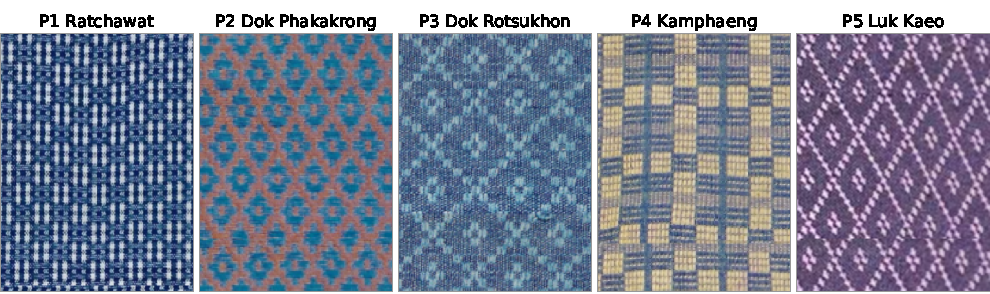
\includegraphics[width=\textwidth]{sic_rect}
\caption{The five photographs after illumination flattening, rotation, affine and perspective correction, cropped as in Fig.~\ref{fig:photos}.}
\label{fig:rect}
\end{figure}

Fig.~\ref{fig:resid} shows what each geometric stage achieves on P1. After the affine stage the residual map is a bowl, low at the centre and high at the edges, the signature of perspective. After the perspective correction the bowl is gone and the map is flat except for the bottom row, where the cloth is folded. After the fold check and re-registration the mean residual has fallen from 0.208 to 0.098, a reduction of 53\%; on P2 it fell from 0.112 to 0.061, a reduction of 46\%, and over the five patterns the reduction is 24\% to 53\%, with the same ordering of the stages on all of them. The local shifts needed in re-registration were 2.2 to 3.7 pixels, which is the amount of non-flatness that a global perspective correction cannot absorb. For P1 to P4 the second, independent estimate of the period agreed with the autocorrelation within 1.3 pixels on both axes. For P5 the vertical estimate was poorly defined, because the photograph holds only three repeats vertically, and lay 6 pixels, or 3\%, below the autocorrelation value; the vertical period of P5 is the least certain number in Table~\ref{tab:geom}.

\begin{figure}[htbp]
\centering
\begin{subfigure}{0.46\textwidth}\centering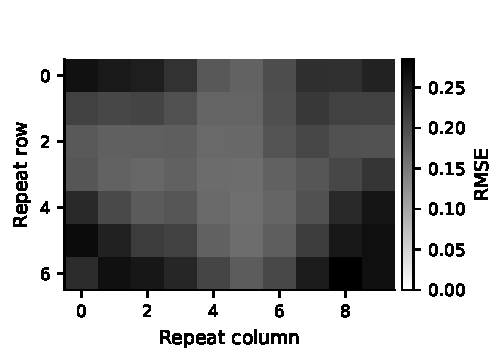
\includegraphics[width=\linewidth]{fig05_a}\caption{P1 after the affine stage}\end{subfigure}\hfill
\begin{subfigure}{0.46\textwidth}\centering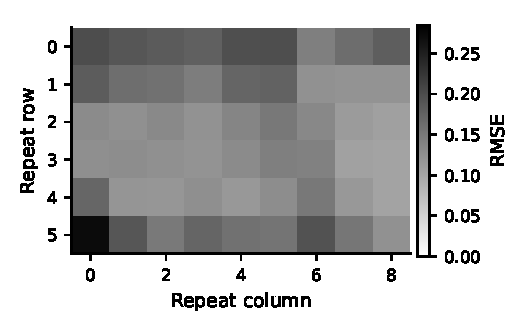
\includegraphics[width=\linewidth]{fig05_b}\caption{P1 after perspective correction}\end{subfigure}\\[2pt]
\begin{subfigure}{0.46\textwidth}\centering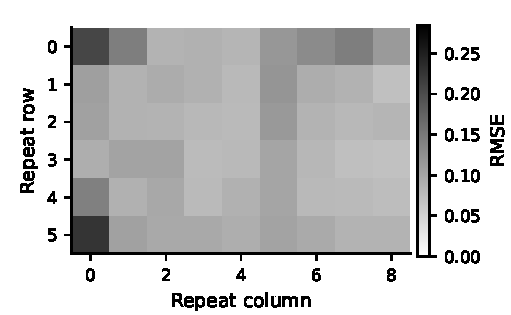
\includegraphics[width=\linewidth]{fig05_c}\caption{P1 after re-registration}\end{subfigure}\hfill
\begin{subfigure}{0.46\textwidth}\centering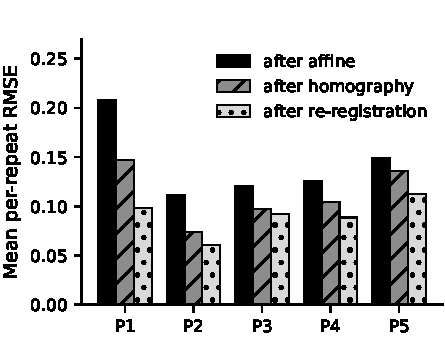
\includegraphics[width=\linewidth]{fig05_d}\caption{Mean residual by stage, all patterns}\end{subfigure}
\caption{Residual maps of P1 (disagreement of each repeat with the average, dark for little) after the affine stage (a), after perspective correction (b) and after re-registration (c), and the mean residual by stage for all patterns (d).}
\label{fig:resid}
\end{figure}

The two rules for finding the repeat were compared on the full images and on crops, with the repeat-finding stage alone run on each crop. On the full images the shortest-vector rule returns the correct repeat, within 3\% of the final value, for P2 only; on P1, P3, P4 and P5 it returns a motif-internal period of 21 by 24, 26 by 27, 34 by 11 and 40 by 65 pixels, and on the twelve crops of each pattern it succeeds on none for those four and on all twelve for P2. The shell rule returns the correct repeat on all five full images and on 12, 12, 10, 12 and 6 of the 12 crops of P1 to P5. The reference repeat is the one found on the full image and confirmed by the second estimate and by the round trips below; there is no independent ground truth for it, but a motif-internal period can be recognised because the pattern does not repeat at that shift. The two patterns whose crops are least stable, P3 and P5, hold the fewest repeats in the field of view.


Fig.~\ref{fig:pre} shows the illumination trend, the rotation search, the lattice anchors and their drift for P5, the most distorted photograph; Fig.~\ref{fig:ac} shows the autocorrelations with the selected repeat vectors, and Fig.~\ref{fig:fold} the fold-residual curves that give the second estimate of the period, with a sharp minimum for P1 to P4 and a nearly flat vertical curve for P5.

\begin{figure}[htbp]
\centering
\begin{subfigure}{0.46\textwidth}\centering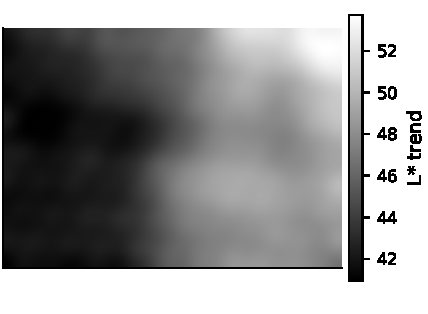
\includegraphics[width=\linewidth]{fig03_a}\caption{Illumination trend of P5}\end{subfigure}\hfill
\begin{subfigure}{0.46\textwidth}\centering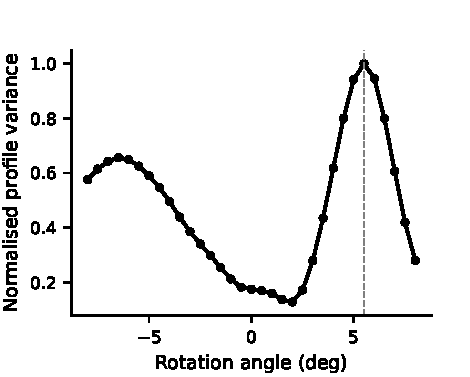
\includegraphics[width=\linewidth]{fig03_b}\caption{Rotation search for P5}\end{subfigure}\\[2pt]
\begin{subfigure}{0.46\textwidth}\centering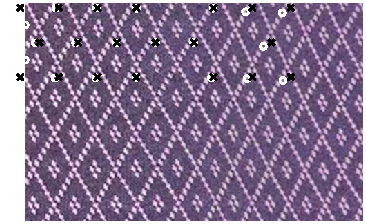
\includegraphics[width=\linewidth]{fig03_c}\caption{Lattice anchors on rectified P5}\end{subfigure}\hfill
\begin{subfigure}{0.46\textwidth}\centering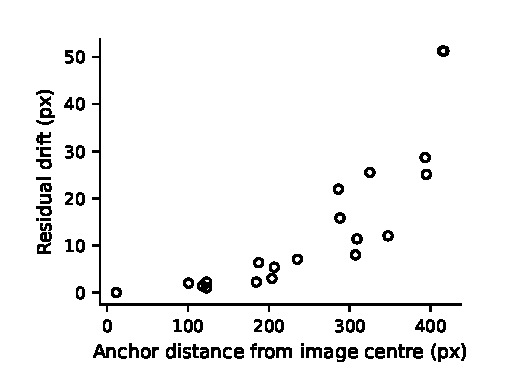
\includegraphics[width=\linewidth]{fig03_d}\caption{Anchor drift against distance from the centre}\end{subfigure}
\caption{Geometry recovery on P5: lighting trend removed (a), rotation search peaking at 5.5 degrees (b), the 35 anchors (c), and anchor drift growing with distance from the centre to 51 pixels (d).}
\label{fig:pre}
\end{figure}

\begin{figure}[htbp]
\centering
\begin{subfigure}{0.46\textwidth}\centering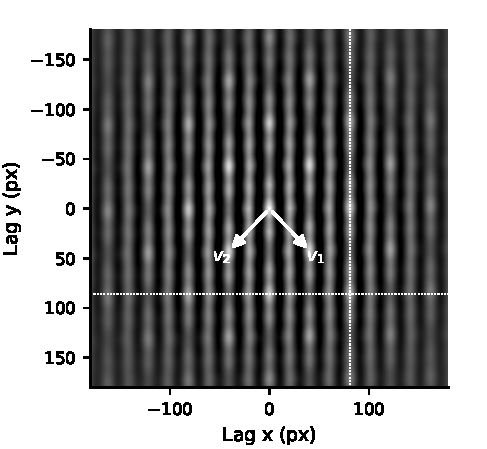
\includegraphics[width=\linewidth]{fig04_a}\caption{P1}\end{subfigure}\hfill
\begin{subfigure}{0.46\textwidth}\centering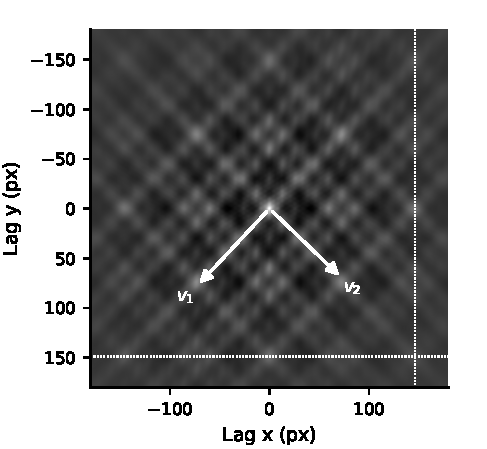
\includegraphics[width=\linewidth]{fig04_b}\caption{P3}\end{subfigure}\\[2pt]
\begin{subfigure}{0.46\textwidth}\centering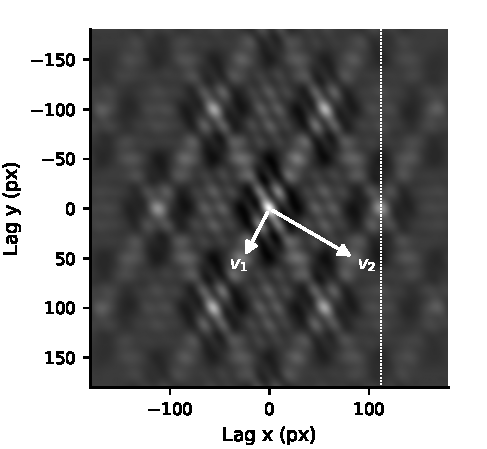
\includegraphics[width=\linewidth]{fig04_c}\caption{P5}\end{subfigure}\hfill
\begin{subfigure}{0.46\textwidth}\centering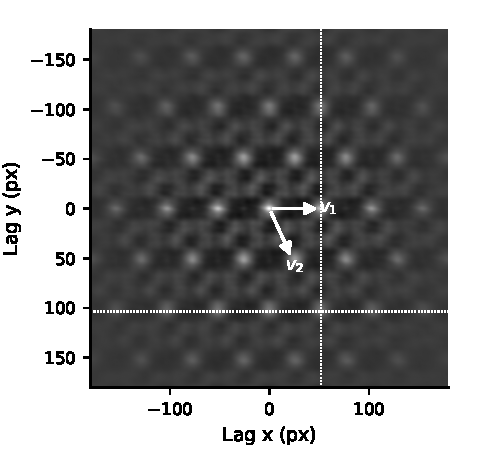
\includegraphics[width=\linewidth]{fig04_d}\caption{P2}\end{subfigure}
\caption{Autocorrelation of the rectified images with the selected repeat vectors, for the three patterns with strong motif-internal peaks, P1, P3 and P5, which the shell rule rejects (a to c), and for the clean diamond lattice of P2 (d).}
\label{fig:ac}
\end{figure}

\begin{figure}[htbp]
\centering
\begin{subfigure}{0.46\textwidth}\centering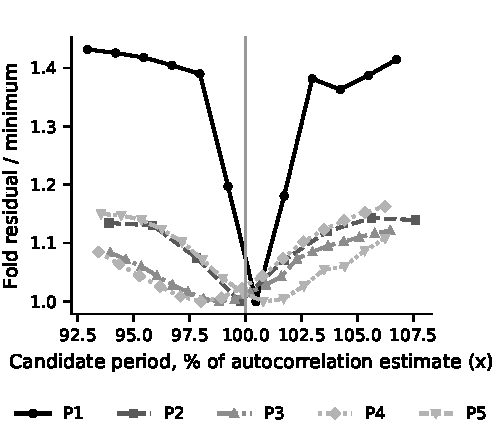
\includegraphics[width=\linewidth]{fig15_a}\caption{Horizontal period}\end{subfigure}\hfill
\begin{subfigure}{0.46\textwidth}\centering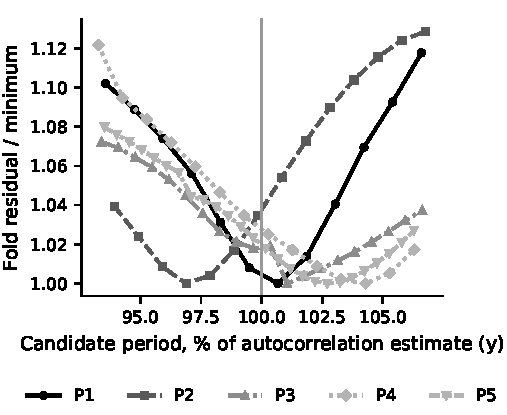
\includegraphics[width=\linewidth]{fig15_b}\caption{Vertical period}\end{subfigure}
\caption{Fold-residual check of the period: disagreement between repeats and their average at each candidate period, relative to the autocorrelation estimate.}
\label{fig:fold}
\end{figure}
\subsection{The tile and the cell draft}

Fig.~\ref{fig:tiles} shows the mean tiles and the measured drafts of the five patterns at one scale. The Ratchawat tile shows the lattice of squares and the dash grid between them, Dok Phakakrong the flower on its diamond lattice, Kamphaeng the wall-like bands, and Luk Kaeo the alternating pair of diamonds that makes its true repeat 111 by 201 pixels rather than the single diamond of half that size. The cell grids are 22 by 12 cells for P1, 13 by 29 for P2, 35 by 36 for P3, 34 by 14 for P4 and 36 by 49 for P5, with cell pitches of 3.1 to 7.4 pixels.

\begin{figure}[htbp]
\centering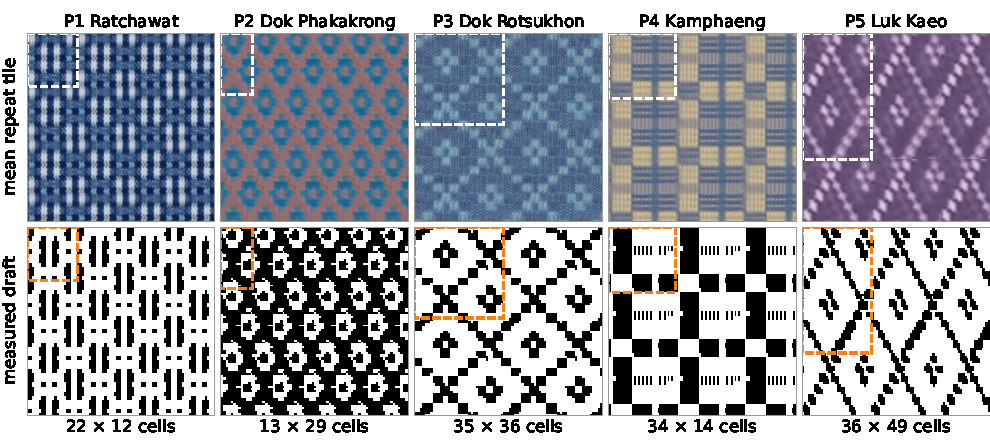
\includegraphics[width=\textwidth]{sic_tiles}
\caption{Mean repeat tiles (top) and measured drafts (bottom), each repeated to fill 300 by 300 pixels so that all are at one scale; the dashed rectangle marks one repeat, black cells are floats.}
\label{fig:tiles}
\end{figure}

Fidelity to the photograph is highest at the scale of the motif, which is what a two-colour draft records. Tiled back over the rectified photograph, the mean colour tile reaches SSIM of 0.50 to 0.83 at motif scale and the two-colour draft 0.39 to 0.79; at pixel level the draft reaches only 0.15 to 0.40, because the photograph carries yarn texture that a two-colour draft does not, and the mean colour difference is 9.8 to 15.7 CIEDE2000 units. Fig.~\ref{fig:recon} shows on P2 that the difference between photograph and draft is concentrated in yarn-level texture. Reducing the tile to four colours instead of two lowers the colour error to 2.1 to 4.0 units, and to six colours 1.6 to 3.0, so a visual archive should keep a four-colour palette beside the two-colour loom draft.

\begin{figure}[htbp]
\centering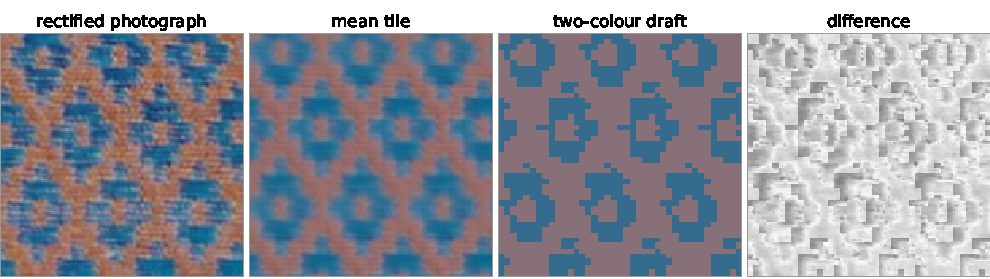
\includegraphics[width=\textwidth]{sic_recon}
\caption{P2 on one crop: rectified photograph, reconstruction from the mean tile, reconstruction from the two-colour draft, and their difference (white for none); the difference lies in yarn texture, not pattern.}
\label{fig:recon}
\end{figure}


Table~\ref{tab:fid} gives the full fidelity measurements. The edge F1 of P2 is zero because its blue and dusty-rose colours have nearly equal lightness, a limitation of a lightness-based measure. The palette error falls from 3.6 to 7.9 CIEDE2000 units at two colours to 1.6 to 3.0 at six, with a knee at three to four colours.

\begin{table}[htbp]
\centering\footnotesize
\caption{Fidelity of the reconstruction to the rectified photograph: SSIM at pixel and motif scale for the mean tile and the two-colour draft, and PSNR, CIEDE2000 colour difference and edge F1 for the draft.}
\label{tab:fid}
\begin{tabular}{lcccccccc}
Id & \multicolumn{2}{c}{SSIM mean tile} & \multicolumn{2}{c}{SSIM two-colour} & PSNR (dB) & $\Delta E_{00}$ mean & $\Delta E_{00}$ 95th & Edge F1 \\
 & pixel & motif & pixel & motif & & & & \\
\midrule
P1 & 0.428 & 0.706 & 0.172 & 0.393 & 13.6 & 15.7 & 45.9 & 0.34 \\
P2 & 0.477 & 0.826 & 0.404 & 0.789 & 19.4 & 12.2 & 32.0 & 0.00 \\
P3 & 0.261 & 0.671 & 0.155 & 0.609 & 19.3 & 9.8 & 22.6 & 0.30 \\
P4 & 0.252 & 0.568 & 0.155 & 0.492 & 18.3 & 11.6 & 28.7 & 0.29 \\
P5 & 0.368 & 0.498 & 0.337 & 0.487 & 16.1 & 10.2 & 31.4 & 0.30 \\
\end{tabular}
\end{table}
\subsection{The loom draft and the weavers' heddle counts}

Table~\ref{tab:draft} and Fig.~\ref{fig:shaft} give the loom analysis, and Fig.~\ref{fig:draft} shows the factored draft of P4. Exact factoring of the measured drafts needs 7, 13, 21, 8 and 36 shafts for P1 to P5, against the weavers' 4, 8, 8, 4 and 4 pattern heddles. The shaft-projection curves in Fig.~\ref{fig:shaft} show why: forcing the drafts of P1 to P4 onto the weaver's count changes only 3.8, 2.9, 2.4 and 3.8\% of their cells, against 10 to 25\% for random drafts of the same size and float density, so the extra shafts come from a few scattered cells, and the curves bend at or below the weaver's count. Luk Kaeo is the exception, at 11.9\% on four shafts and 4.3\% even on sixteen: its diagonals of single floats make every column distinct at the cell scale, because the weaver produces them with a twill-like threading of single threads that a cell of 3.1 by 4.1 pixels does not resolve. The projection curve flags this, which the fidelity measures do not. Longest floats are 3 to 12 cells along picks and 7 to 16 along ends; the 16-cell float of P2 is the bar of the flower, bound in practice by the ground weave. Mirror agreement is 93 to 98.5\% for P1, P3 and P4 and 84 to 87\% for P2 and P5, whose alternating motifs break the mirror at the cell level.

\begin{table}[htbp]
\centering
\setlength{\tabcolsep}{2pt}\scriptsize
\caption{Loom analysis: cells in the repeat (ends by picks), cell pitch, pattern shafts and treadles of the measured and regularised drafts, weaver's heddle count, projection cost at that count for each draft and for a random draft of equal size and density, and mirror agreement of the measured draft.}
\label{tab:draft}
\begin{tabular}{lllrrrrrrrrrr}
Id & Cells & Pitch & \multicolumn{2}{c}{Measured} & \multicolumn{2}{c}{Regularised} & Hed- & \multicolumn{3}{c}{Cost at weaver's count (\%)} & Mirror & Mirror \\
 & & (px) & shafts & treadles & shafts & treadles & dles & meas. & reg. & random & V (\%) & H (\%) \\
\midrule
P1 & 22 $\times$ 12 & 3.6 $\times$ 7.1 & 7 & 5 & 5 & 3 & 4 & 3.8 & 3.0 & 17.1 & 98.5 & 98.5 \\
P2 & 13 $\times$ 29 & 3.9 $\times$ 3.4 & 13 & 21 & 5 & 6 & 8 & 2.9 & 0.0 & 10.2 & 86.2 & 83.6 \\
P3 & 35 $\times$ 36 & 4.1 $\times$ 4.0 & 21 & 20 & 10 & 8 & 8 & 2.4 & 1.1 & 20.1 & 95.4 & 93.2 \\
P4 & 34 $\times$ 14 & 3.1 $\times$ 7.4 & 8 & 6 & 5 & 3 & 4 & 3.8 & 3.4 & 24.9 & 95.8 & 97.5 \\
P5 & 36 $\times$ 49 & 3.1 $\times$ 4.1 & 36 & 43 & 14 & 19 & 4 & 11.9 & 10.2 & 20.6 & 87.3 & 85.3 \\
\end{tabular}
\end{table}

\begin{figure}[htbp]
\centering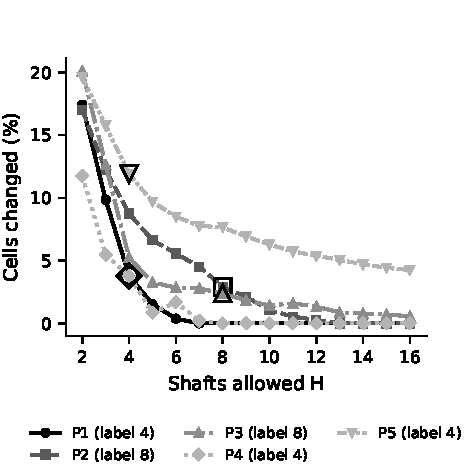
\includegraphics[width=0.6\textwidth]{fig10_a}
\caption{Shaft projection cost of the measured drafts: cells changed when each draft is forced onto 2 to 16 shafts; the open marker is the weaver's heddle count.}
\label{fig:shaft}
\end{figure}

\begin{figure}[htbp]
\centering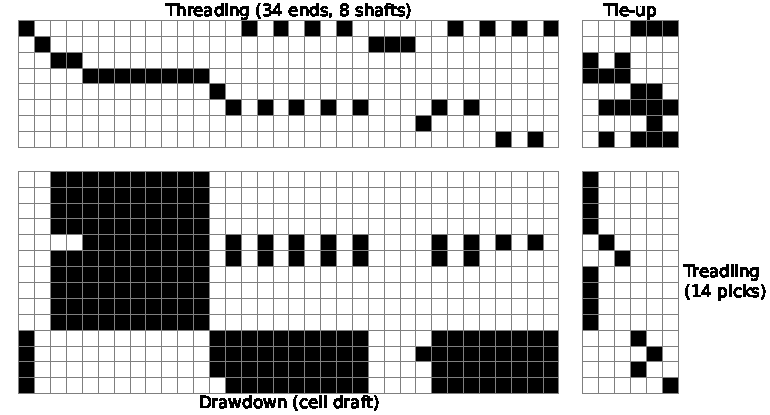
\includegraphics[width=\textwidth]{fig08_draft}
\caption{Weaving draft of P4 factored from the measured draft: threading (top), tie-up (top right), treadling (right) and drawdown, which equals the cell draft.}
\label{fig:draft}
\end{figure}

\subsection{The symmetry interpretation}

Fig.~\ref{fig:sym} shows for every pattern the tile, the measured draft, the regularised draft and the cells that changed, and Table~\ref{tab:draft} the effect on the loom draft. All three mirror and rotation operations met the 80\% agreement rule on every pattern, with agreements of 80.4 to 98.5\%, and the half-repeat shift on P1 with 100\%. Regularisation changed 0.8, 9.8, 3.8, 2.5 and 7.4\% of the cells of P1 to P5, isolated cells on motif edges rather than parts of motifs. The shafts needed fall from 7, 13, 21, 8 and 36 to 5, 5, 10, 5 and 14, and the treadles from 5, 21, 20, 6 and 43 to 3, 6, 8, 3 and 19. Against the weavers' counts, Ratchawat and Kamphaeng now need 5 shafts against 4, Dok Rotsukhon 10 against 8, Dok Phakakrong 5 against 8, and Luk Kaeo 14 against 4; the cost of projecting the regularised drafts onto the weavers' counts is 3.0, 0.0, 1.1, 3.4 and 10.2\%. Dok Phakakrong's regularised draft needs 5 shafts where the weaver used 8; the record flags the difference so that the weaver can say whether the cell grid of 13 by 29 merges threading classes that are kept separate on the loom. The motif-scale fidelity to the photograph changes by at most 0.013.

A noise test shows what the regularisation removes. The difference between the averaged tile and its mirror or rotation was compared, cell by cell, with the variation expected from averaging the repeats: the departures from symmetry exceed that variation by a factor of 1.7 to 28, and 3 to 65\% of cells depart significantly at the 1\% level, most on P1 and P2 and least on P4. The averaging therefore resolves structure finer than its own noise, whether that structure is the irregularity of a hand-woven cloth or a residual of the photograph, and the two drafts keep the two kinds of information apart: the measured draft records the cloth as photographed, and the regularised draft, with a tie-up two to nine times smaller, is the simpler draft for the weaver to accept or reject. The values for each operation are given in Table~\ref{tab:symnoise}.

\begin{figure}[htbp]
\centering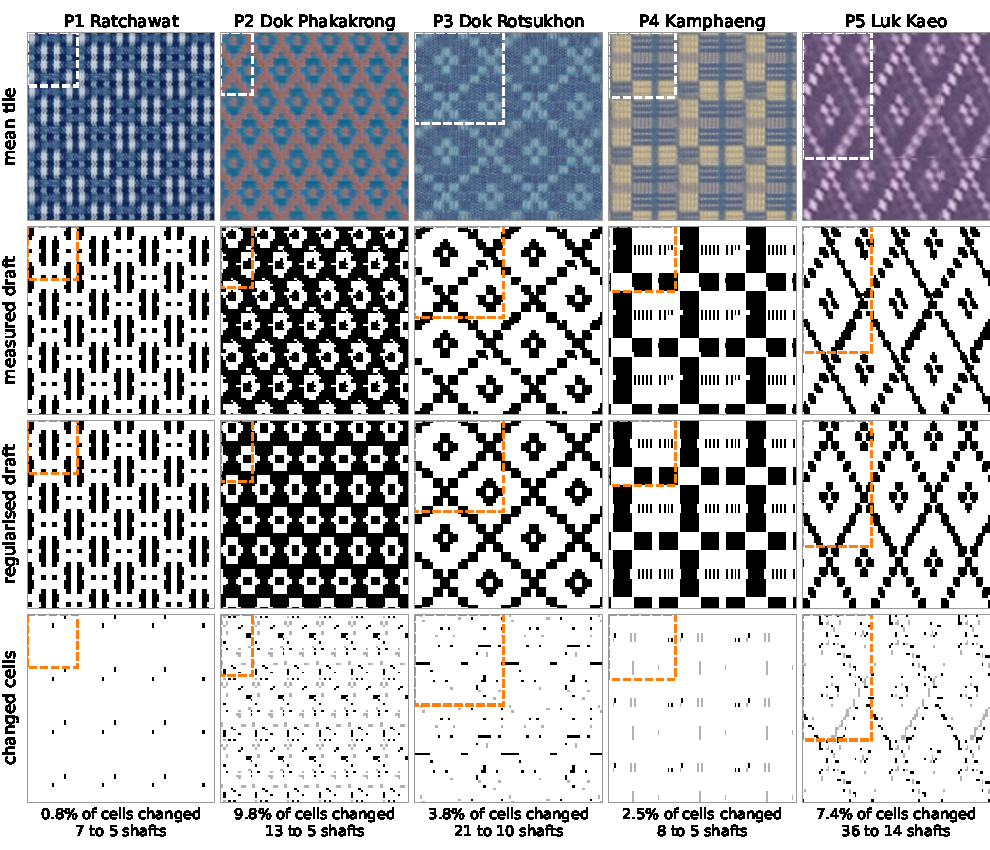
\includegraphics[width=\textwidth]{sic_sym}
\caption{Symmetry interpretation at one scale: mean tile, measured draft, regularised draft, and cells changed (black added, grey removed); the dashed rectangle marks one repeat.}
\label{fig:sym}
\end{figure}


In detail, for each pattern the cell-lightness tile $L$ was compared with its transform $T(L)$ under each symmetry operation. The variance of the averaged tile at each cell was estimated as the variance across the $n$ registered repeats divided by $n$, and the statistic at each cell is $(L - T(L))^2$ divided by the sum of that variance at the cell and at its image. Table~\ref{tab:symnoise} gives the mean of the statistic over cells, which would be about 1 if the departures were averaging noise, and the percentage of cells above the 1\% quantile of a chi-square distribution with one degree of freedom. Cells are spatially correlated, so the percentages are indicative rather than exact. A simpler form of the test that divides by the variance across single repeats, without the factor $n$, gives values between 0.06 and 0.32; the values with the factor $n$ show that the averaging resolves departures from symmetry finer than its own noise, whether these come from the cloth or from residuals of the photograph.

\begin{table}[htbp]
\centering\small
\caption{Symmetry noise test: registered repeats, and for each operation the mean statistic and the percentage of cells significant at the 1\% level.}
\label{tab:symnoise}
\begin{tabular}{lccccc}
Id & Repeats & Vertical mirror & Horizontal mirror & Two-fold rotation & Half shift \\
\midrule
P1 & 54 & 10.3 / 35 & 10.5 / 44 & 14.6 / 45 & 0.0 / 0 \\
P2 & 57 & 23.8 / 61 & 15.4 / 52 & 27.6 / 65 & -- \\
P3 & 10 & 2.0 / 7 & 3.7 / 16 & 4.2 / 18 & -- \\
P4 & 18 & 1.9 / 6 & 1.7 / 3 & 2.7 / 11 & -- \\
P5 & 16 & 5.2 / 19 & 5.9 / 19 & 3.0 / 11 & -- \\
\end{tabular}
\end{table}
\subsection{Tests on artificial cloth and on crops of the photographs}

Fig.~\ref{fig:rt} shows the round trips on artificial cloth rendered from the extracted drafts. Over the fifteen cases the repeat was recovered with a median error of 0.12 pixels and a maximum of 0.97 pixels, the applied tilt was recovered to within the 0.1 degree resolution of the search in every case, and the draft, after resampling the recovered pixel draft onto the known cell grid at the best alignment, agreed with the known draft on 99.8 to 100\% of cells, exactly 100\% in all twelve cases of P1 to P4 and 99.8 to 99.9\% for P5, whose 36 by 49 cell draft loses one to three cells at a pitch of 3 pixels. The cell grid itself was recovered exactly in 13 of 15 cases; in two P4 cases the search returned a 34 by 7 grid, half the true height. The P4 cell draft is not periodic at half height, so these two cases are counted as misses of the grid search, which stopped at the half-height harmonic, although the recovered pixel-level draft, resampled onto the known 34 by 14 grid, still agreed on every cell. The round trips establish that the extraction stage itself is exact to a fraction of a pixel and a handful of cells; the uncertainty that remains on real cloth comes from the photograph, and is measured by the crop stability below.

\begin{figure}[htbp]
\centering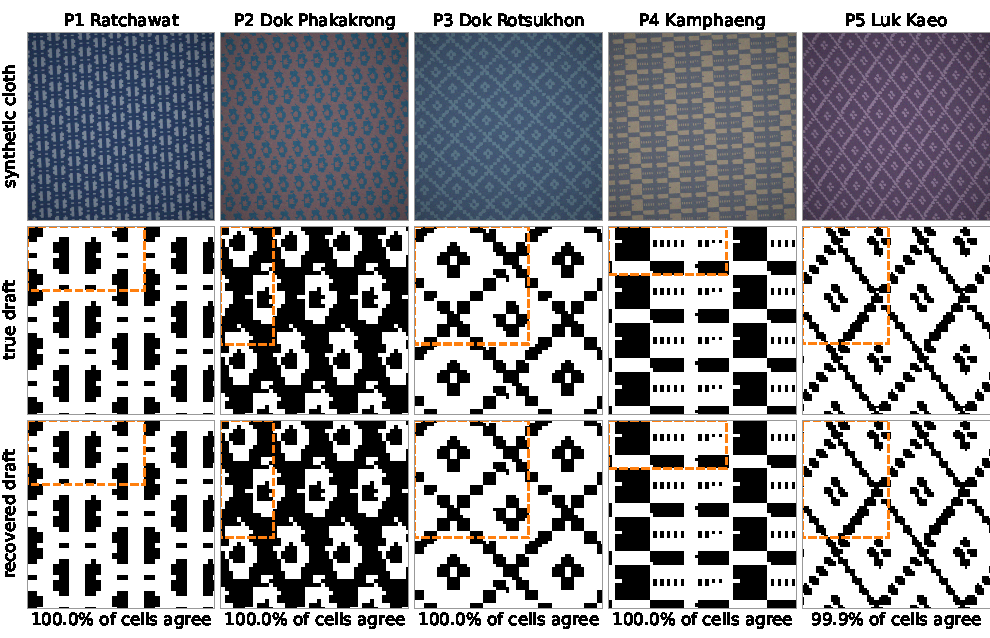
\includegraphics[width=\textwidth]{sic_rt}
\caption{Round trips: artificial cloth rendered from each draft (tilt 2.5 degrees, noise), the known draft, and the draft recovered by the whole method, with the percentage of cells that agree.}
\label{fig:rt}
\end{figure}

The synthetic resolution sweep covered the 17 of 30 pattern-and-pitch combinations whose repeat fits within the 160-pixel search limit of the method. The repeat period was recovered to within 0.35 pixels in every case except P3 at 4 pixels per cell, where the error was 0.78 pixels; the cell draft agreed with the known draft on 95.8 to 100\% of cells; and the cell grid itself was recovered exactly in every case at 4 pixels per cell or more, in 3 of 5 patterns at 3 pixels, and never at 2 pixels. The practical floor is therefore 3 to 4 pixels per pattern cell, which the five photographs just meet. The noise sweep kept the draft at 99.2\% agreement or better up to a noise level far above that of the photographs.

Fig.~\ref{fig:boot} shows the crop stability, in which the whole method, including the perspective correction, is run on each crop; the counts differ from the repeat-finding comparison above because the perspective correction on a small crop rests on fewer anchors. For P1 to P4, nine of the twelve crops of each returned a repeat within 3\% of the full-image value, with median deviations of 2.0 to 2.5\%; for P5 only four did, with a median deviation of 3.4\% and a vertical spread of 23 pixels, because an 80\% crop of P5 holds only 2.5 repeats vertically and the vertical period is then not identifiable. P3, whose crops hold 2.6 repeats vertically, also gave one outlying crop that locked onto a sub-lattice. The crops of P1, P2 and P4 hold at least 3.2 repeats along each axis and were stable. P5 is also the most oblique photograph and has the largest repeat, but the data point to the number of repeats in the frame as the cause, and the guidance below is drawn from it.

\begin{figure}[htbp]
\centering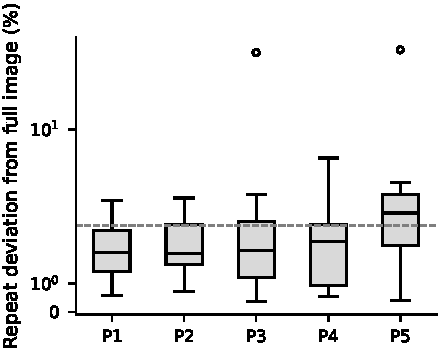
\includegraphics[width=0.6\textwidth]{fig11_a}
\caption{Crop stability: repeat found on each of twelve random 80\% crops as a percentage of the full-image repeat. P1 to P4 are stable; P5, with fewer than three repeats vertically in a crop, is not.}
\label{fig:boot}
\end{figure}


Fig.~\ref{fig:rtdetail} gives the repeat, draft agreement and tilt recovered in the fifteen round trips, and Fig.~\ref{fig:sweep} the resolution and noise sweeps together with the draft from the smoothness prior on P5. Without the search for the cell-grid origin the same fifteen round trips recovered the exact grid in 2 cases only, both of P2, with grids such as 36 by 12 for P1 and 29 by 37 for P5.

\begin{figure}[htbp]
\centering
\begin{subfigure}{0.46\textwidth}\centering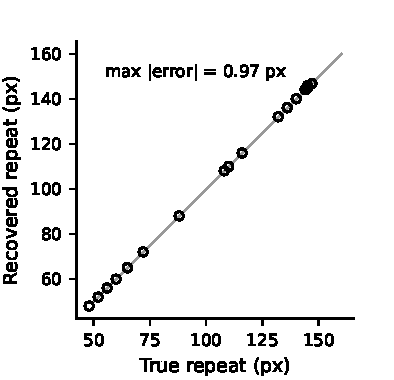
\includegraphics[width=\linewidth]{fig12_b}\caption{Recovered against true repeat}\end{subfigure}\hfill
\begin{subfigure}{0.46\textwidth}\centering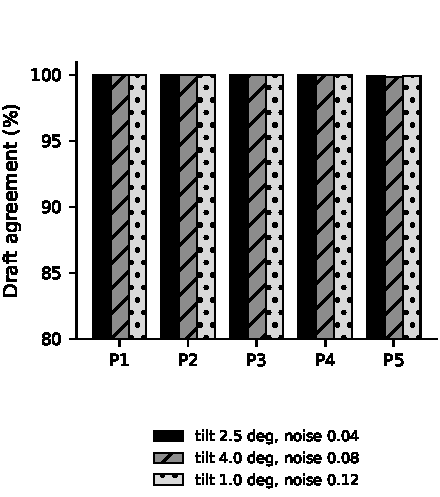
\includegraphics[width=\linewidth]{fig12_c}\caption{Draft agreement}\end{subfigure}\\[2pt]
\begin{subfigure}{0.46\textwidth}\centering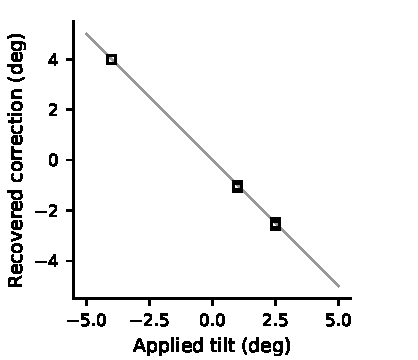
\includegraphics[width=\linewidth]{fig12_d}\caption{Recovered tilt}\end{subfigure}
\caption{Round-trip measurements on artificial cloth rendered from the extracted drafts, three cases per pattern.}
\label{fig:rtdetail}
\end{figure}

\begin{figure}[htbp]
\centering
\begin{subfigure}{0.46\textwidth}\centering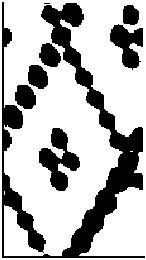
\includegraphics[width=\linewidth,height=1.9in,keepaspectratio]{fig17_a}\caption{P5 measured draft}\end{subfigure}\hfill
\begin{subfigure}{0.46\textwidth}\centering
\includegraphics[width=\linewidth,height=1.9in,keepaspectratio]{fig17_b}\caption{P5 draft with smoothness prior}\end{subfigure}\\[2pt]
\begin{subfigure}{0.46\textwidth}\centering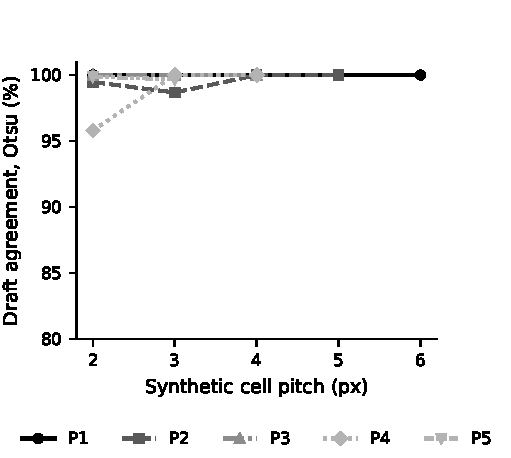
\includegraphics[width=\linewidth]{fig17_c}\caption{Draft agreement against synthetic pitch}\end{subfigure}\hfill
\begin{subfigure}{0.46\textwidth}\centering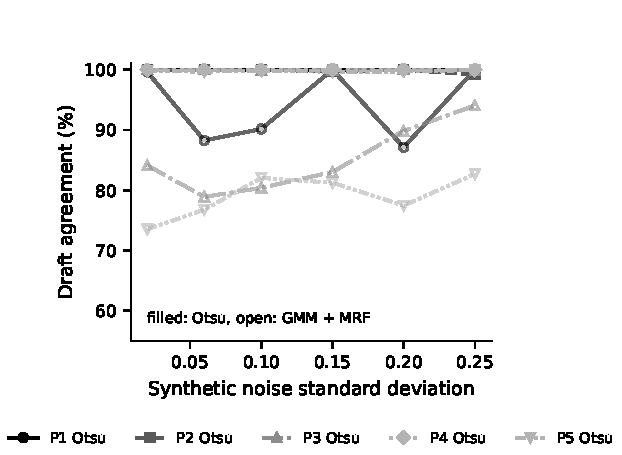
\includegraphics[width=\linewidth]{fig17_d}\caption{Draft agreement against noise}\end{subfigure}\\[2pt]
\begin{subfigure}{0.46\textwidth}\centering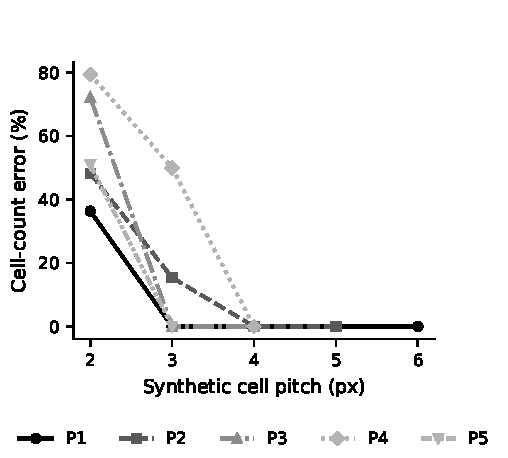
\includegraphics[width=\linewidth]{fig17_e}\caption{Cell-count error against pitch}\end{subfigure}\hfill
\begin{subfigure}{0.46\textwidth}\centering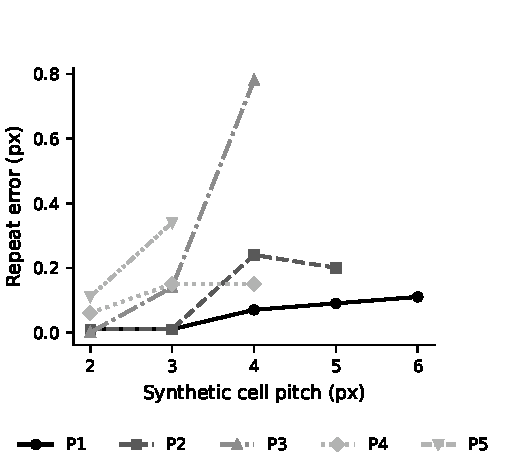
\includegraphics[width=\linewidth]{fig17_f}\caption{Repeat error against pitch}\end{subfigure}
\caption{P5 measured draft and draft with a smoothness prior (a, b), and the synthetic resolution and noise sweeps (c to f).}
\label{fig:sweep}
\end{figure}
\subsection{Further techniques evaluated}

Table~\ref{tab:notadopted} summarises the nine further techniques. The structural rules outperformed every learned alternative on these cloths: the shell rule beat the machine-learned selector, which chose a double-size lattice on all twelve crops of Ratchawat and was correct on 19 of 30 synthetic crops against 28 for the rule; re-registered averaging beat the Noise2Noise denoiser, whose tiles were 18 to 56\% less sharp; and the plain threshold beat the draft with a smoothness prior, which merged the single-cell floats of P5 and fell to 74 to 79\% agreement on synthetic cloth where the threshold stayed above 99\%. The displacement vote map, designed for printed fabric with strong motifs, found the repeat on 15 of 60 crops. Registration super-resolution from the repeats raised the number of patterns whose cell grid was recovered exactly at 3 pixels per cell on synthetic cloth from 3 to 4 of 5 and gave Kamphaeng a draft on exactly the weaver's four shafts; on the other patterns it gave different cell grids and more shafts than the mean tile, so it is kept as an option, and the disagreement between the two tiles is itself a useful measure of how uncertain the cell count is. The per-cell uncertainty estimate flags 0.4 to 2.4\% of cells as worth a second look; the texture distance, homogeneity score and shape descriptors add checks and an index to the archive.

\begin{table}[htbp]
\caption{Further techniques evaluated, their purpose and outcome.}
\label{tab:notadopted}
\small
\renewcommand{\arraystretch}{1.1}
\begin{tabular}{L{3.6cm}L{3.2cm}L{5.4cm}L{2.2cm}}
Technique & Purpose & Outcome on the five cloths & Adopted \\ \midrule
Machine-learned repeat selector \citep{friedman2001} & Choose the repeat & Confident wrong lattice on P1; 19 of 30 synthetic crops against 28 for the rule & No \\
Noise2Noise denoiser \citep{lehtinen2018} & Cleaner tile & 18 to 56\% less sharp than averaging & No \\
Draft with smoothness prior \citep{besag1986} & Cleaner draft & Merges single-cell floats; 74 to 79\% on synthetic P3 and P5 & No \\
Displacement vote map \citep{xiang2022,qu2020} & Find the repeat & Repeat found on 15 of 60 crops against 51 for autocorrelation in the same run & No \\
Registration super-resolution \citep{irani1991,ayyurek2026} & Finer tile & Exact grid at 3 pixels per cell in 4 of 5 synthetic cases against 3; different cell grids on all real cloths & Optional \\
Per-cell uncertainty \citep{kuo2004} & Where to look & 0.4 to 2.4\% of cells flagged & Diagnostic \\
Texture distance, homogeneity \citep{gatys2015,liu2015} & Misalignment-tolerant check & Drafts as close to the tile as the cloth is to itself & Diagnostic \\
Shape descriptors \citep{hu1962} & Archive index & Separates nine of the ten pairs of patterns & Index only \\
\end{tabular}
\end{table}


A gradient-boosted classifier scores candidate lattices from the same shell features the rule uses, trained on 30 synthetic crops rendered from the extracted drafts with random tilt, noise and cropping; a hybrid falls back to the rule below a probability of 0.5. On the real crops the selector matches the rule on P2 and P4 and loses one crop on P3 and P5, but on P1 it chooses a 102 by 105 pixel double-size lattice on all twelve crops with a confidence of 0.72; leave-one-pattern-out on synthetic crops it is correct on 19 of 30 against 28 for the rule.


Against the individual repeats at motif scale the mean reaches SSIM of 0.68 to 0.90, the median 0.70 to 0.90 and the denoiser 0.64 to 0.89, lower on every pattern, and the denoiser is 18 to 56\% less sharp. The median is 6 to 21\% sharper than the mean at equal SSIM and is kept in the archive beside it.


The mixture draft with the Ising prior disagrees with the measured draft on 5 to 19\% of pixels, and Fig.~\ref{fig:sweep}a and b show why on P5: the prior merges the single-cell floats of the diagonals into bands. In the synthetic noise sweep the measured draft agrees with the true draft to 99.2 to 100\% for noise from 0.02 to 0.25, while the mixture draft falls to 78.9\% on P3 and 73.5\% on P5.

Fig.~\ref{fig:advtiles} shows for each pattern the mean tile up-sampled by cubic interpolation, the super-resolved tile from 10 to 57 registered repeats and the per-cell uncertainty map. The sub-pixel shifts between repeats had a root mean square of 0.13 to 6.5 pixels. The super-resolved mean is 2 to 8\% less sharp than the re-registered mean, because registration residuals blur it as much as the finer grid sharpens it, but the super-resolved median is 4 to 16\% sharper. On synthetic cloth the super-resolved tile recovered the exact cell grid in 4 of 5 patterns at 3 pixels per cell against 3 of 5 for the mean tile, and neither did at 2 pixels. On the real cloth the super-resolved tile yields cell grids of 30 by 17, 17 by 28, 56 by 35, 29 by 20 and 36 by 54, different from the mean-tile grids on every pattern, and its regularised drafts need 7, 7, 13, 4 and 26 shafts at a cost of 4.3, 0.0, 1.0, 0.0 and 11.3\% at the weaver's count, reaching the weaver's count exactly on P4.

The displacement vote map is dominated by yarn-scale peaks on P3 and shows no lattice; on twelve crops per pattern it succeeded on 12, 3, 0, 0 and 0 against 12, 12, 10, 11 and 6 for the autocorrelation, and fused with it on 12, 11, 0, 0 and 1. The per-cell uncertainty estimate flags 0.4 to 2.4\% of cells, with mean confidence 0.86 to 0.97, and on P5 these cells lie along the diagonals. The texture distance of the two-colour reconstructions to the tile, 0.1 to 1.2 thousandths, is of the same order as that of a single repeat, 0.2 to 0.9 thousandths; the homogeneity score is 0.030 to 0.095, lowest for Dok Phakakrong and highest for Luk Kaeo. The Hu moments of the regularised drafts separate every pair of patterns by 1.9 or more units in at least one moment except P2 and P5, which differ by at most 0.7.


\begin{figure}[htbp]
\centering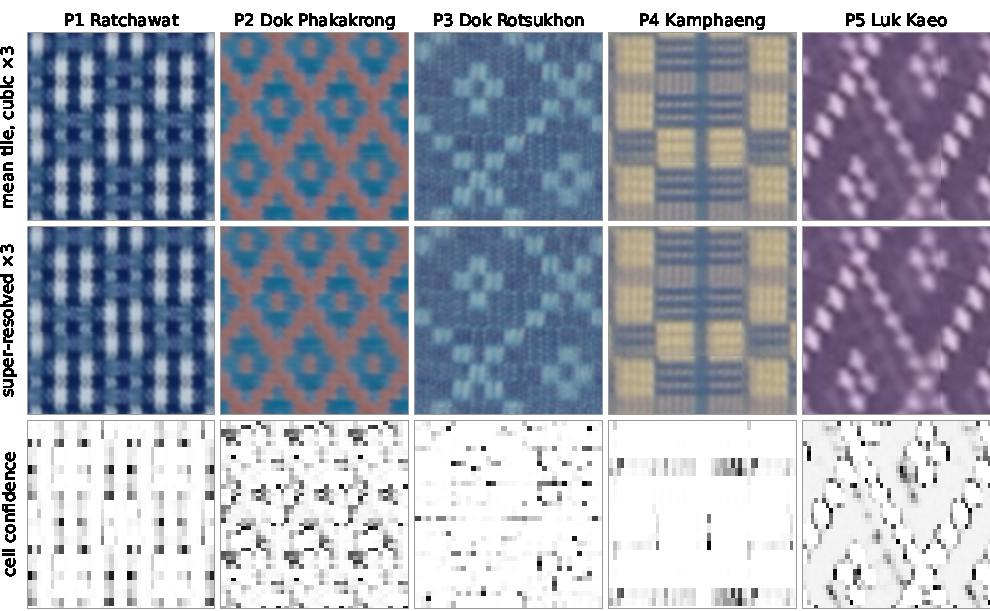
\includegraphics[width=\textwidth]{sic_sr}
\caption{Mean tile up-sampled three times, super-resolved tile from the registered repeats, and per-cell uncertainty map (white for confident), at one scale.}
\label{fig:advtiles}
\end{figure}
\section{Discussion}

\subsection{Use of the record in conservation practice}

The record separates into a part that is checked and a part that is bounded. The checked part is the geometry and the repeat: tilt, shear and perspective are removed with the cloth's own lattice, the period is confirmed by two independent estimates and is stable across crops when the frame holds enough repeats, and the mean tile reproduces the pattern at motif scale. A conservator can use this part now, to record the repeat size and the pattern of a piece, to compare the pattern of two pieces or of a piece and a photograph in a database, and to produce a clean colour tile for publication or for briefing a weaver. The bounded part is the cell draft and the shaft count derived from it. The extraction is not the limit, since the draft is recovered almost exactly from artificial cloth; the photograph is, resolving the pattern cell at 3 to 7 pixels and the individual threads not at all. The draft is therefore a pattern-cell draft, not a thread draft: the number of warp ends and picks in a cell is not measured, and a WIF or TC2 file with one end per cell gives the pattern at cell resolution and must be scaled by the thread count per cell, which a conservator can obtain with a thread counter on the cloth, before it is woven. No cloth has yet been woven from these files, and that trial, with the weaver's judgement as the final check, is the next step.

A reading rule follows from the measurements and is set out in Table~\ref{tab:rule}. The most severe category that applies wins, the measured draft is the one evaluated, and the thresholds are provisional, drawn from these five cases. Under it, Ratchawat, Dok Rotsukhon and Kamphaeng are ready for use; Dok Phakakrong is ready apart from the symmetry interpretation, which differs from its measured draft on 9.8\% of cells and proposes fewer shafts than the weaver used, so it goes to the weaver; and Luk Kaeo needs a closer photograph, which its own projection curve and crop instability say. Where no weaver's count is available, the shafts needed by the measured and regularised drafts are compared instead, and a record whose two drafts differ by more than 5\% of cells is treated as one to check. In practice the method runs with one command on a laptop from the open code, and its outputs are image and WIF files that any weaving software opens.

\begin{table}[htbp]
\caption{Reading rule for a record and the placement of the five patterns; the most severe row that applies wins, and the thresholds are provisional.}
\label{tab:rule}
\small
\renewcommand{\arraystretch}{1.1}
\begin{tabular}{L{2.6cm}L{8.6cm}L{2.9cm}}
Reading & Criteria, all measured on the record itself & Patterns \\ \midrule
Ready for use & Nine or more of twelve crops within 3\% of the full-image repeat; the two period estimates agree within 2\%; projection cost at the weaver's count below 5\%; regularised and measured drafts differ on 5\% of cells or less & P1, P3, P4 \\
Confirm with the weaver & Projection cost 5 to 10\%, or the regularised draft needs fewer shafts than the weaver's count, or the two drafts differ on more than 5\% of cells & P2 \\
Closer photograph needed & Fewer than three repeats along an axis, or crops disagree, or projection cost above 10\% & P5 \\
\end{tabular}
\end{table}

\subsection{The heddle counts and the symmetry interpretation}

The weaver's heddle count is the one piece of information in this study that does not come from the photograph. A projection cost of a few percent at that count, where random drafts cost 10 to 25\%, is consistent with the digitised structure being the one the weaver set up, and the comparison is conditional on the cell grid, since the super-resolved tile gives a different grid and a different count on every pattern. Disagreement is informative in both directions. More shafts than the weaver's count, with a projection curve that bends at that count, means scattered cells that a loom would not need, as on P1, P3 and P4. Many more shafts with a curve that does not bend, as on P5, means that the photograph does not resolve the structure. Fewer shafts than the weaver's count, as on P2 after regularisation, means that the cell grid may be coarser than the weaver's threading. Each case calls for a different action, and the record states which; a weaving trial with the weavers, who hold the final judgement, is the natural next step.

The two drafts serve two readers. The measured draft keeps the small departures from symmetry that the averaging resolves, which on the two patterns with alternating motifs, P2 and P5, amount to 13 to 16\% of cells; the regularised draft, stored beside it with the list of cells it changed, gives the weaver the simpler threading to confirm or correct.

\subsection{Summary of the method against usual practice}

Table~\ref{tab:novelty} sets the components of the method against usual practice and the evidence reported above. Structural rules read from the cloth account for nearly all of the gain, and for heritage documentation, where ground truth is rare, this is a practical advantage: every stage of the method is a rule that a conservator can inspect.

\begin{table}[htbp]
\caption{Components of the method compared with usual practice, with the evidence reported in this paper.}
\label{tab:novelty}
\small
\renewcommand{\arraystretch}{1.15}
\begin{tabular}{L{2.4cm}L{3.3cm}L{4.2cm}L{4.4cm}}
Problem & Usual practice & This work & Evidence \\ \midrule
Finding the repeat & Two shortest autocorrelation peaks \citep{liu2004pami} & Shell rule over the first and second lattice shells & Correct on 5 of 5 cloths and 52 of 60 crops, against 1 of 5 and 12 of 60 for the usual rule \\[5pt]
Geometry of a hand photograph & Calibration target, flat-bed scan or manual correction & Affine and perspective correction from the cloth's own lattice, fold check and per-repeat re-registration & Residual between repeats reduced by 24\% to 53\%; two independent period estimates agree within 1.3 pixels on four patterns \\[5pt]
Cell draft & Pixel threshold with one pixel per thread assumed & Search for the cell grid and its origin & Known drafts recovered with 99.8\% to 100\% agreement and the exact grid in 13 of 15 round trips, against 2 of 15 without the origin search \\[5pt]
Draft consistency & None, so scattered cells add shafts & Regularised draft stored beside the measured draft, with a noise test & Shafts needed reduced from between 7 and 36 to between 5 and 14; both drafts kept \\[5pt]
Trust in the record & Visual comparison & Checks against the photograph, crops, artificial cloth and the weaver's heddle count, with a reading rule & Four drafts project onto the weaver's count at a cost of 2.4\% to 3.8\% of cells, against 10\% to 25\% for random drafts; the fifth is sent for a closer photograph \\
\end{tabular}
\end{table}

\subsection{Scope}

The five patterns are five case studies on new cloth in good condition from one community, photographed by the authors, and the method assumes a periodic pattern on a cloth flat enough to show several repeats. Within that scope the results are consistent across all five, and the structure the method relies on, a two-colour cell draft on a periodic lattice, is shared by supplementary-weft traditions across Southeast Asia, which are the natural next test, together with a second photograph of each pattern by a different person and a weaving trial. Historic pieces from collections bring soiling, loss, creases and fragility that the five cloths did not; for them the method should be run on a photograph taken under the object's own handling rules, without flattening, and the crop stability and residual maps will show whether the condition of the piece still allows a repeat to be read. The cell-to-thread ratio, which the method does not measure, is a one-line entry with a thread counter in the field record.

\subsection{Guidance for photographing a cloth}

Table~\ref{tab:capture} turns the results into guidance for a conservator or a community member in the field. Two numbers matter most: at least four repeats of the pattern in each direction, and at least four pixels across one pattern cell. Both can be judged at the camera: the repeat should span no more than a quarter of the frame in each direction, and a single float should be clearly visible when the picture is viewed at full size. A photograph of 4000 pixels width that frames 40 cm of cloth gives 10 pixels per millimetre, so a pattern cell one millimetre wide spans 10 pixels; when framing and resolution conflict, two photographs, one of the whole and one closer, serve better than a compromise. The field checklist is therefore short: frame four or more repeats, fill the frame with the cloth from square-on, use even light without flash, and place a ruler and a colour reference beside the cloth. The evidence column states what each item rests on.

\begin{table}[htbp]
\caption{Guidance for photographing a cloth for pattern documentation, with the evidence from this study.}
\label{tab:capture}
\small
\renewcommand{\arraystretch}{1.1}
\begin{tabular}{L{2.6cm}L{6.0cm}L{5.9cm}}
Aspect & Recommendation & Evidence \\ \midrule
Framing & At least four repeats of the pattern along each axis; more is better & Crops of the five cloths: fewer than three repeats along an axis unstable (P5, partly P3), at least 3.2 stable \\
Resolution & At least four pixels across one pattern cell, three at the limit; use the camera's full resolution and no digital zoom & Synthetic sweep: exact cell grid at four pixels per cell and above, at three in 3 of 5 patterns, never at two \\
Thread-level detail & Not needed for the cell draft; for a thread-exact record use a flat-bed scanner or macro lens at about 12 or more pixels per thread, and note the threads per cell with a thread counter & Thread recognisers need about 12 pixels per thread \citep{meng2021}; the five photographs resolve cells, not threads \\
Angle & As square-on as possible; moderate tilt is corrected & Five cloths: rotation of up to 5.5 degrees and perspective drift of up to 51 pixels removed; P5, the most oblique, is the least certain \\
Flatness and condition & Lay the cloth flat on a neutral surface, without pins or tension, within what its condition allows; a slight fold is tolerated; do not flatten brittle, flaking or heavily creased pieces & One cloth: fold on P1 absorbed by the fold check and re-registration; aged cloth not yet tested \\
Lighting & Diffuse, even light without flash; avoid shadows across the cloth; if pattern and ground are close in lightness, add a photograph under raking light & Five cloths: vignetting and fold shadow removed; synthetic noise tolerated far above camera noise; P2's palette of equal lightness defeats the edge check \\
Colour and scale & Place a colour reference and a ruler beside the cloth, outside the pattern area & Recommended practice; not used by the method, but they give the archive true colour and the physical size of the repeat \\
Record with the photograph & Pattern name, weaver, heddle count, threads per cell, place and date; keep the unedited original file & Recommended practice; the heddle count is the independent check of the draft used throughout this paper \\
\end{tabular}
\end{table}

\section{Conclusions}

A method was presented that turns a hand-held photograph of Koh Yo cloth into a pattern tile and a cell-level weaving draft in loom formats, and that checks the record against the photograph, against itself, against artificial cloth and against the weaver's heddle count. On five patterns the repeat was found on every cloth, the disagreement between repeats fell by 24\% to 53\%, and four drafts project onto the weavers' stated heddle counts at a cost of 2.4\% to 3.8\% of cells, far below chance, while the checks sent the fifth for a closer photograph. The method needs no equipment beyond a camera, runs in seconds, and every stage of it can be inspected. Its drafts are pattern-cell drafts, ready for scaling by the thread count and for confirmation by the weavers, and the five cases reported here open a route that other supplementary-weft traditions can follow. The code, the photographs and the loom files are released openly so that others can test it on theirs.


\section{Acknowledgements}
The authors thank the weavers of Koh Yo for the cloths, the pattern names and the heddle counts, and the Office of Academic Resources of Prince of Songkla University for the southern information database.

\section{Disclosure statement}
No potential conflict of interest was reported by the authors.

\section{Funding}
\sloppy
This work was supported by the Ratchadaphiseksomphot Endowment Fund, Chulalongkorn University, Journal Research Grant in Arts and Humanities, Grant No. RSF-AnH-69-10-25-05.

\section{Data availability statement}
The code, the five photographs, the results files from which every number in this paper is read, the figure scripts and the loom files (WIF, TC2 TIFF and point-paper charts) are openly available at \url{https://github.com/cnnitipong/kohyo-pattern-digitisation}.

\bibliographystyle{sic}
\bibliography{refs}
\end{document}
